% Provenance (never printed): see sources/outline_sources.md (Year 1: insolation with
% latitude and season, the radiative surplus and deficit, meridional heat transport by
% the atmosphere and the ocean, latent heat). Exercise and problem values in the Book 3
% scratch calculator calc/ch27.py; figures from figdata/bachelor-1/insolation.py (Kepler
% orbit of _solar.py) and energy_balance.py (NCEP-NCAR Reanalysis 1, long-term means
% 1991-2020, datasets bachelor-1-ncep-*).
% Physics owns the inverse-square law, the black body and the Stefan-Boltzmann law, the
% seasons and latent heat (recalled). Book 2 (g10) gave the quarter of the solar constant,
% the global budget diagram and its closure, latent and sensible heat in words, the
% annual-mean insolation curve and the poleward transport in words: re-founded here with
% derivations and data. Ch. 1 gave the instantaneous insolation, the declination and the
% rising and setting of the Sun.
\chapter{Radiación y transporte de calor}\label{ch:b1:radiation-heat-transport}

Desde un millón de millas de distancia, la cara iluminada de la Tierra es un disco de mar azul, tierra parda y nube blanca. La luz del sol cae más directamente sobre el centro del disco, cerca de los trópicos, y roza sus bordes; los trópicos absorben mucha más energía que las regiones polares. Sin embargo, los trópicos no se calientan año tras año, ni los polos se enfrían. Los vientos y las corrientes oceánicas llevan el exceso hacia los polos, varios petavatios de él. Este capítulo mide los tres términos de ese balance: la luz solar que recibe cada \omterm{def:b1:spherical-astronomy:geographic}{latitud}, la parte que retiene y el infrarrojo que devuelve al espacio, y el transporte que cubre la diferencia. Una parte grande del transporte viaja en una forma invisible, como vapor de agua, cuyo calor latente se libera donde se condensa en lluvia.
% ledger: commons:epic-earth, trenberth:transport

\begin{omfigure}
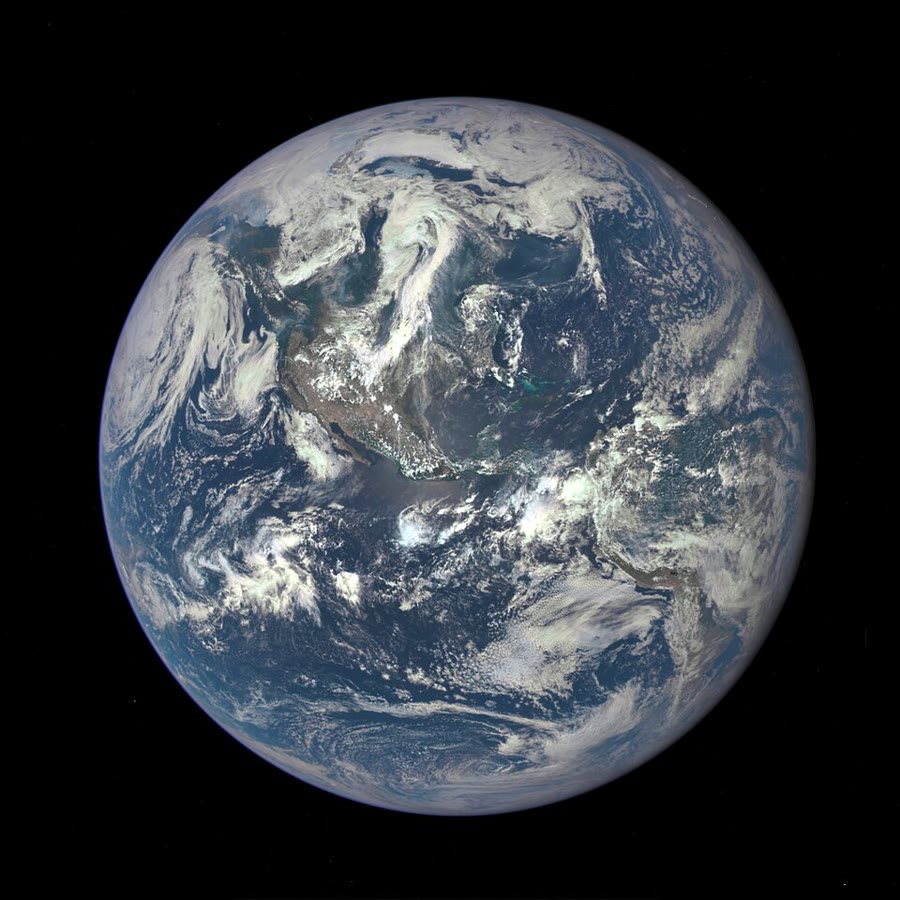
\includegraphics[width=0.55\linewidth]{images/book3/b1-epic-earth.jpg}

{\small La cara iluminada entera de la Tierra, fotografiada el 6 de julio de 2015 por una cámara del Deep Space Climate Observatory, a un millón de millas; Norteamérica y Centroamérica están en el centro, con los mares someros turquesa del Caribe. Dos semanas después del solsticio de junio, el Ártico, arriba, está iluminado todo el día. Las nubes brillantes reflejan buena parte de la luz que les llega; el tinte azulado es luz solar dispersada por las moléculas del aire. (NASA Goddard Space Flight Center, dominio público, vía Wikimedia Commons.)}
\label{fig:b1:radiation-heat-transport:epic}
\end{omfigure}
% ledger: commons:epic-earth (polar day: figdata/bachelor-1/insolation.py)

\begin{recall}
\Cref{ch:b1:spherical-astronomy} definió la \omterm{def:b1:spherical-astronomy:insolation}{insolación}, la potencia de la luz solar recibida por metro cuadrado de una superficie horizontal en el tope de la atmósfera, $I = S_0(a/r)^2\sin h_\odot$ mientras el Sol está sobre el horizonte, con $S_0 = \qty{1361}{W.m^{-2}}$
a la distancia media $a$; dio la altura del Sol a partir de su \omterm{def:b1:spherical-astronomy:equatorial}{ángulo horario} $H$, su \omterm{def:b1:spherical-astronomy:equatorial}{declinación} $\delta$ y la \omterm{def:b1:spherical-astronomy:geographic}{latitud} $\varphi$,
$\sin h_\odot = \sin\varphi\sin\delta + \cos\varphi\cos\delta\cos H$; y el \omterm{def:b1:spherical-astronomy:equatorial}{ángulo horario} $H_0$ de la puesta, $\cos H_0 = -\tan\varphi\tan\delta$
(\cref{prop:b1:spherical-astronomy:rising}). \Cref{ch:b1:comparative-planetology} definió el \omterm{def:b1:comparative-planetology:albedo}{albedo de Bond} de un planeta y su \omterm{def:b1:comparative-planetology:equilibrium-temperature}{temperatura de equilibrio}. Los libros de física dan la ley del inverso del cuadrado para la luz, la radiación de un cuerpo negro,
$\sigma T^4$ por metro cuadrado con $\sigma = \qty{5.670e-8}{W.m^{-2}.K^{-4}}$
(Stefan--Boltzmann), y el calor latente de un cambio de estado. El libro 2 mostró que la Tierra intercepta en promedio una cuarta parte de la constante solar, dibujó el balance energético global de la Tierra y comprobó que cuadra, y describió con palabras el transporte de calor hacia los polos.
% ledger: earth:TSI, const:sigma, ipcc:budget-toa
\end{recall}

\section{Insolación según la latitud y la estación}\label{sec:b1:radiation-heat-transport:insolation}

La \omterm{def:b1:spherical-astronomy:insolation}{insolación} instantánea cambia de minuto en minuto a medida que el Sol cruza el cielo. Para el clima, lo que cuenta es su suma a lo largo de un día.

\begin{definition}[Insolación media diaria]\label{def:b1:radiation-heat-transport:daily-insolation}
La \emph{insolación media diaria}\index{insolación media diaria} $\bar Q$ a una \omterm{def:b1:spherical-astronomy:geographic}{latitud} en un día dado es la \omterm{def:b1:spherical-astronomy:insolation}{insolación} instantánea promediada sobre las 24 horas de ese día, con las noches incluidas, manteniendo la \omterm{def:b1:spherical-astronomy:equatorial}{declinación} del Sol y su distancia en sus valores del día. Es una potencia por metro cuadrado de superficie horizontal en el tope de la atmósfera, en \unit{W.m^{-2}}.
\end{definition}

Mantener $\delta$ y $r$ fijos durante un día es inocuo: la \omterm{def:b1:spherical-astronomy:equatorial}{declinación} cambia como mucho \ang{0.4} al día, y la distancia menos de un \qty{0.03}{\percent}.
% ledger: earth:obliquity, earth:ecc (computed in figdata/bachelor-1/insolation.py)

\begin{theorem}[Insolación media diaria]\label{thm:b1:radiation-heat-transport:daily}
A la \omterm{def:b1:spherical-astronomy:geographic}{latitud} $\varphi$, en un día en que la \omterm{def:b1:spherical-astronomy:equatorial}{declinación} del Sol es $\delta$ y su distancia $r$,
\[
  \bar Q = \frac{S_0}{\pi}\left(\frac{a}{r}\right)^{2}
  \bigl(h_0\sin\varphi\sin\delta + \cos\varphi\cos\delta\sin h_0\bigr),
\]
donde $h_0 \in [0, \pi]$ es el \omterm{def:b1:spherical-astronomy:equatorial}{ángulo horario} de la puesta en radianes: $\cos h_0 =
-\tan\varphi\tan\delta$ cuando $|\tan\varphi\tan\delta| \le 1$; $h_0 = \pi$ en el día
polar ($\tan\varphi\tan\delta > 1$); $h_0 = 0$, y $\bar Q = 0$, en la noche
polar ($\tan\varphi\tan\delta < -1$).
\end{theorem}

\begin{proof}
La hora angular $H$ avanza uniformemente a lo largo de $2\pi$ en un día, así que la media del día es la media sobre $H \in [-\pi, \pi]$. El Sol está sobre el horizonte para $-h_0 < H < h_0$,
donde $\sin h_\odot > 0$, y la \omterm{def:b1:spherical-astronomy:insolation}{insolación} es nula en otro caso. Por tanto
\[
  \bar Q = \frac{1}{2\pi}\int_{-h_0}^{h_0} S_0\left(\frac{a}{r}\right)^{2}
  \bigl(\sin\varphi\sin\delta + \cos\varphi\cos\delta\cos H\bigr)\,\mathrm dH ,
\]
que es $(S_0/2\pi)(a/r)^2\bigl(2h_0\sin\varphi\sin\delta +
2\cos\varphi\cos\delta\sin h_0\bigr)$.
Los límites provienen de \cref{prop:b1:spherical-astronomy:rising}: la altura es cero cuando $\cos H = -\tan\varphi\tan\delta$. Si ese número supera 1 en valor absoluto, el Sol nunca cruza el horizonte: cuando $\tan\varphi\tan\delta > 1$, el integrando es positivo para todo $H$ y la integral recorre todo el día, $h_0 = \pi$; cuando $\tan\varphi\tan\delta < -1$, es negativo para todo $H$ y el Sol nunca sale.
\end{proof}

Dos casos especiales conviene saberlos de memoria. En el ecuador, $\varphi = 0$ y
$h_0 = \pi/2$ sea cual sea la estación:
\[
  \bar Q_\text{ecuador} = \frac{S_0}{\pi}\left(\frac{a}{r}\right)^{2}\cos\delta ,
\]
mayor en los equinoccios, $S_0/\pi = \qty{433.2}{W.m^{-2}}$ a la distancia media.
En un polo en su verano, $h_0 = \pi$ y $\varphi = \pi/2$: $\bar Q_\text{polo} =
S_0(a/r)^2\sin\delta$, con el Sol dando vueltas por el cielo a una altura constante igual a la \omterm{def:b1:spherical-astronomy:equatorial}{declinación}.
% ledger: earth:TSI

\begin{proposition}[El verano polar]\label{prop:b1:radiation-heat-transport:polar-summer}
En un día de \omterm{def:b1:spherical-astronomy:equatorial}{declinación} $\delta > 0$, la \omterm{def:b1:radiation-heat-transport:daily-insolation}{insolación media diaria} en el Polo Norte
supera a la del ecuador si y solo si $\pi\tan\delta > 1$, es decir, $\delta >
\ang{17.66}$. En el solsticio de junio, $\delta = \ang{23.44}$, el cociente es $\pi\tan
\delta = 1.362$.
\end{proposition}

\begin{proof}
Los dos casos especiales de arriba comparten el factor $(S_0/\pi)(a/r)^2$; su cociente es
$\pi\sin\delta/\cos\delta = \pi\tan\delta$, que supera 1 cuando $\tan\delta >
1/\pi$, $\delta > \arctan(1/\pi) = \ang{17.66}$. Con la oblicuidad,
$\pi\tan\ang{23.44} = 1.362$.
\end{proof}
% ledger: earth:obliquity

Con la órbita de la Tierra, el solsticio de junio cae cerca del afelio, $(a/r)^2 = 0.968$:
el Polo Norte recibe entonces \qty{524}{W.m^{-2}} como media diaria, el ecuador
\qty{385}{W.m^{-2}}. Seis meses después el Polo Sur, cerca del perihelio, recibe
\qty{559}{W.m^{-2}}, un \qty{6.7}{\percent} más que el Polo Norte en su verano: el cociente es exactamente el de los dos valores de $(a/r)^2$. La figura siguiente
muestra $\bar Q$ a lo largo de un año completo. Los máximos están en los polos en los solsticios;
las cuñas oscuras son las noches polares, limitadas por la \omterm{def:b1:spherical-astronomy:geographic}{latitud} $\ang{90} -
|\delta|$; el punto subsolar, donde el Sol pasa por el cénit al mediodía, se mueve entre los trópicos con la \omterm{def:b1:spherical-astronomy:equatorial}{declinación}.
% ledger: earth:TSI, earth:ecc, earth:obliquity, nasa:earth-perihelion-longitude, usno:seasons-2026 (computed in figdata/bachelor-1/insolation.py)

\begin{omfigure}
\begin{tikzpicture}
\begin{axis}[omrecord, width=0.8\linewidth, height=6.4cm, view={0}{90},
  xmin=0, xmax=365, ymin=-90, ymax=90, xlabel={día del año (desde el 1 de enero)},
  ylabel={latitud (\unit{\degree})}, xtick={0,60,...,360}, ytick={-90,-60,...,90},
  colormap/viridis, colorbar, point meta min=0, point meta max=560,
  colorbar style={ylabel={$\bar Q$ (\unit{W.m^{-2}})}, ytick={0,100,...,500}, width=0.3cm},
  axis on top, grid=none]
% figdata/bachelor-1/insolation.py; ledger: earth:TSI, earth:ecc, earth:obliquity, nasa:earth-perihelion-longitude, usno:tropical-year, usno:seasons-2026
\addplot3[surf, shader=interp, mesh/ordering=y varies, mesh/rows=73]
  table[x=day, y=lat, z=Q] {figdata/out/bachelor-1-insolation-grid.dat};
\addplot3[white, dashed, line width=0.8pt] table[x=day, y=decl, z expr=600] {figdata/out/bachelor-1-insolation-sun.dat};
\addplot3[white, line width=0.6pt, unbounded coords=jump] table[x=day, y=night_n, z expr=600] {figdata/out/bachelor-1-insolation-sun.dat};
\addplot3[white, line width=0.6pt, unbounded coords=jump] table[x=day, y=night_s, z expr=600] {figdata/out/bachelor-1-insolation-sun.dat};
\node[font=\scriptsize, text=white] at (axis cs:28,81,700) {noche polar};
\node[font=\scriptsize, text=white] at (axis cs:172,-81,700) {noche polar};
\node[font=\scriptsize, text=white, anchor=south] at (axis cs:172,26,700) {latitud subsolar};
\end{axis}
\end{tikzpicture}

{\small \omterm{def:b1:radiation-heat-transport:daily-insolation}{Insolación media diaria} en el tope de la atmósfera frente al día del año y la \omterm{def:b1:spherical-astronomy:geographic}{latitud}, a partir de \cref{thm:b1:radiation-heat-transport:daily} con $S_0 = \qty{1361}{W.m^{-2}}$ y la órbita de la Tierra. Discontinua: la \omterm{def:b1:spherical-astronomy:geographic}{latitud} subsolar, igual a la \omterm{def:b1:spherical-astronomy:equatorial}{declinación}; continua: los bordes de las noches polares. Los polos de verano reciben más que cualquier otro lugar de la Tierra; el verano austral, cerca del perihelio, es el más brillante de los dos.}
\label{fig:b1:radiation-heat-transport:matrix}
\end{omfigure}
% ledger: earth:TSI, earth:ecc, earth:obliquity, nasa:earth-perihelion-longitude, usno:seasons-2026

Promediando $\bar Q$ a lo largo del año se obtiene la \omterm{def:b1:spherical-astronomy:insolation}{insolación} media anual de cada \omterm{def:b1:spherical-astronomy:geographic}{latitud} (figura siguiente): \qty{415.6}{W.m^{-2}} en el ecuador, \qty{328.3}{W.m^{-2}} a \ang{40}, \qty{172.4}{W.m^{-2}} en cada polo. El verano polar es intenso, pero el invierno polar es oscuro, y a lo largo de un año el ecuador recibe \num{2.41} veces lo que un polo. La curva es la misma en los dos hemisferios, aunque el verano austral es el más brillante; \cref{exo:b1:radiation-heat-transport:10} muestra por qué.
% ledger: earth:TSI, earth:ecc, earth:obliquity (computed in figdata/bachelor-1/insolation.py)

\begin{omfigure}
\begin{tikzpicture}
\begin{axis}[omrecord, width=0.8\linewidth, height=5.6cm, xmin=-90, xmax=90, ymin=0, ymax=600,
  xlabel={latitud (\unit{\degree})}, ylabel={$\bar Q$ (\unit{W.m^{-2}})},
  xtick={-90,-60,...,90}, ytick={0,100,...,600}]
% figdata/bachelor-1/insolation.py; ledger: earth:TSI, earth:ecc, earth:obliquity, nasa:earth-perihelion-longitude
\addplot[omThm, line width=0.8pt] table[x=lat, y=Q_jun] {figdata/out/bachelor-1-insolation-annual.dat};
\addplot[omDef, line width=0.8pt] table[x=lat, y=Q_dec] {figdata/out/bachelor-1-insolation-annual.dat};
\addplot[black, line width=1.1pt] table[x=lat, y=Q_ann] {figdata/out/bachelor-1-insolation-annual.dat};
\addplot[black!60, dashed, domain=-90:90] {340.30};
\node[font=\scriptsize, text=omThm, anchor=west] at (axis cs:50,540) {solsticio de junio};
\node[font=\scriptsize, text=omDef, anchor=east] at (axis cs:-50,575) {solsticio de diciembre};
\node[font=\scriptsize, anchor=north] at (axis cs:-72,160) {media anual};
\node[font=\scriptsize, text=black!60, anchor=south west] at (axis cs:-88,342) {media global};
\end{axis}
\end{tikzpicture}

{\small \omterm{def:b1:radiation-heat-transport:daily-insolation}{Insolación media diaria} frente a la \omterm{def:b1:spherical-astronomy:geographic}{latitud} en los dos solsticios, y su media anual (negra). La media anual supera a la media global, \qty{340.3}{W.m^{-2}} (discontinua), entre \ang{37} S y \ang{37} N, en el \qty{60}{\percent} de la superficie de la Tierra.}
\label{fig:b1:radiation-heat-transport:annual}
\end{omfigure}
% ledger: earth:TSI, earth:ecc, earth:obliquity (computed in figdata/bachelor-1/insolation.py)

\begin{proposition}[La media global]\label{prop:b1:radiation-heat-transport:global}
En cada instante, la \omterm{def:b1:spherical-astronomy:insolation}{insolación} promediada sobre toda la esfera es $\tfrac14
S_0(a/r)^2$. Promediada también a lo largo del año, es $S_0/(4\sqrt{1 - e^2})$, donde $e$ es la excentricidad de la órbita: \qty{340.30}{W.m^{-2}} para la Tierra, a menos de un \qty{0.02}{\percent} de $S_0/4 = \qty{340.25}{W.m^{-2}}$.
\end{proposition}

\begin{proof}
La Tierra, de radio $R$, intercepta la luz solar que atraviesa un disco de área $\pi
R^2$, una potencia $S_0(a/r)^2\pi R^2$, que cae en el hemisferio diurno; repartida sobre toda la superficie $4\pi R^2$, da el primer resultado. El promedio temporal de
$(a/r)^2$ a lo largo de la órbita es $1/\sqrt{1-e^2}$
(\cref{exo:b1:radiation-heat-transport:11}).
\end{proof}
% ledger: earth:TSI, earth:ecc

\section{Radiación absorbida y emitida}\label{sec:b1:radiation-heat-transport:toa}

De la luz solar que recibe una \omterm{def:b1:spherical-astronomy:geographic}{latitud}, refleja de vuelta al espacio una fracción, desde nubes, nieve, hielo, desierto y, en menor grado, el mar; absorbe el resto, en el aire y en la superficie. También pierde energía emitiendo radiación infrarroja al espacio, de día y de noche.

\begin{definition}[Radiación de onda larga saliente]\label{def:b1:radiation-heat-transport:olr}
La \emph{radiación de onda larga saliente}\index{radiación de onda larga saliente} (OLR) es la potencia de la radiación infrarroja que sale del tope de la atmósfera hacia el espacio, por metro cuadrado. La \emph{temperatura de emisión}\index{temperatura de emisión}
$T_e$ es la temperatura de un cuerpo negro que emitiría la misma potencia: $\sigma T_e^4 = \text{OLR}$.
\end{definition}

La OLR viene en parte de la superficie, a través del aire donde es transparente al infrarrojo, y en parte del aire y de las cimas de las nubes más arriba. La \omterm{def:b1:radiation-heat-transport:olr}{temperatura de emisión} es una propiedad de la radiación, no la temperatura de un nivel concreto: es más baja que la del suelo de debajo, porque las capas emisoras son más frías.
% ledger: ipcc:budget-surface, ipcc:budget-toa

\begin{definition}[Radiación neta; excedente y déficit radiativos]\label{def:b1:radiation-heat-transport:net-radiation}
La \emph{radiación neta}\index{radiación neta} en el tope de la atmósfera es
\[
  R = \underbrace{(1 - \alpha)\,\bar Q}_{\text{solar absorbida}} - \text{OLR},
\]
donde $\alpha$ es el albedo local, la fracción de la luz solar incidente reflejada
hacia el espacio; las tres magnitudes son medias anuales en una \omterm{def:b1:spherical-astronomy:geographic}{latitud}. Una \omterm{def:b1:spherical-astronomy:geographic}{latitud} donde
$R > 0$ tiene un \emph{excedente radiativo}\index{excedente radiativo}; una donde $R < 0$
tiene un \emph{déficit radiativo}\index{déficit radiativo}.
\end{definition}

Sobre toda la Tierra la \omterm{def:b1:radiation-heat-transport:net-radiation}{radiación neta} debe promediar casi cero, ya que el planeta no se calienta ni se enfría más de unas décimas de vatio por metro cuadrado: la última evaluación sitúa el desequilibrio en \qty{0.7}{W.m^{-2}}, sobre una entrada de \qty{340}{W.m^{-2}} de la que \qty{100}{W.m^{-2}} se reflejan (un albedo global de \num{0.294}) y \qty{239}{W.m^{-2}} salen como infrarrojo.
% ledger: ipcc:budget-toa, earth:albedo

Los perfiles zonales de este capítulo proceden de un reanálisis, es decir, de un sistema de predicción meteorológica ejecutado sobre las últimas décadas, que asimila las observaciones de cada día y entrega un estado completo y coherente de la atmósfera. El reanálisis usado aquí, desde 1948, da medias mensuales en una malla de 94 \omterm{def:b1:spherical-astronomy:geographic}{latitudes} y 192 longitudes; este capítulo usa sus promedios de 1991--2020. Sus flujos de radiación son salidas del modelo, previsiones sujetas a las observaciones. La figura siguiente muestra sus medias zonales frente a $\sin\varphi$, de modo que anchuras iguales en el eje son áreas iguales en la esfera.
% ledger: psl:ncep-r1, kalnay96:reanalysis, data:b3-ncep

\begin{omfigure}
\begin{tikzpicture}
\begin{axis}[omrecord, width=0.8\linewidth, height=6cm, xmin=-1, xmax=1, ymin=0, ymax=320,
  xlabel={latitud (\unit{\degree}, eje en $\sin\varphi$)}, ylabel={flujo (\unit{W.m^{-2}})},
  xtick={-0.866,-0.5,0,0.5,0.866}, xticklabels={60 S,30 S,0,30 N,60 N},
  ytick={0,50,...,300}]
% figdata/bachelor-1/energy_balance.py; ledger: data:b3-ncep, psl:ncep-r1
\addplot[name path=asr, omProp, line width=1pt] table[x expr={sin(\thisrow{lat})}, y=asr] {figdata/out/bachelor-1-energy_balance-toa.dat};
\addplot[name path=olr, omThm, line width=1pt] table[x expr={sin(\thisrow{lat})}, y=olr] {figdata/out/bachelor-1-energy_balance-toa.dat};
\addplot[omProp!25] fill between[of=asr and olr, split, every segment no 1/.style={omDef!18}, every segment no 2/.style={omProp!30}, every segment no 3/.style={omDef!18}];
\node[font=\scriptsize, text=omProp!80!black] at (axis cs:-0.55,300) {solar absorbida};
\node[font=\scriptsize, text=omThm] at (axis cs:-0.2,226) {OLR};
\node[font=\scriptsize] at (axis cs:0,262) {excedente};
\node[font=\scriptsize] at (axis cs:0.86,178) {déficit};
\node[font=\scriptsize] at (axis cs:-0.86,178) {déficit};
\end{axis}
\end{tikzpicture}

{\small Media zonal y anual de la radiación solar absorbida (naranja) y de la \omterm{def:b1:radiation-heat-transport:olr}{radiación de onda larga saliente} (roja) en el tope de la atmósfera, a partir del NCEP-NCAR Reanalysis~1, medias de 1991--2020 (datos proporcionados por NOAA PSL, Boulder, Colorado, EE. UU., desde su sitio web en https://psl.noaa.gov). Sombreado: el \omterm{def:b1:radiation-heat-transport:net-radiation}{excedente radiativo} de las bajas \omterm{def:b1:spherical-astronomy:geographic}{latitudes} y los déficits de las altas \omterm{def:b1:spherical-astronomy:geographic}{latitudes}.}
\label{fig:b1:radiation-heat-transport:toa}
\end{omfigure}
% ledger: data:b3-ncep, psl:ncep-r1, kalnay96:reanalysis

Las dos curvas tienen formas muy distintas. La luz solar absorbida cae desde \qty{288}{W.m^{-2}} cerca del ecuador hasta \qty{76}{W.m^{-2}} a \ang{81} N, en un factor de \num{3.8}: la \omterm{def:b1:spherical-astronomy:insolation}{insolación} baja, y el albedo sube de \num{0.31} a \num{0.57}, con el Sol bajo, la nieve y el hielo marino. La OLR baja solo de \qty{245}{W.m^{-2}} a \qty{192}{W.m^{-2}}, en un factor de \num{1.27}; las \omterm{def:b1:radiation-heat-transport:olr}{temperaturas de emisión} son \qty{256}{K} y \qty{241}{K}. La OLR es incluso algo más baja en el ecuador, \qty{245}{W.m^{-2}}, que cerca de \ang{20}, \qty{269}{W.m^{-2}}: las nubes del cinturón ecuatorial de lluvias se elevan mucho y sus cimas frías emiten poco, mientras que los cielos subtropicales más despejados dejan escapar más infrarrojo. Allí donde la luz solar absorbida supera a la OLR, la \omterm{def:b1:spherical-astronomy:geographic}{latitud} tiene un excedente.
% ledger: data:b3-ncep (values computed in figdata/bachelor-1/energy_balance.py)

\begin{example}[El balance global del reanálisis]\label{ex:b1:radiation-heat-transport:global}
Promediado sobre el globo, el reanálisis recibe \qty{341.9}{W.m^{-2}}, refleja
\qty{117.0}{W.m^{-2}} (un albedo de \num{0.342}), absorbe \qty{224.8}{W.m^{-2}} y
emite \qty{237.7}{W.m^{-2}}: una \omterm{def:b1:radiation-heat-transport:net-radiation}{radiación neta} de \qty{-12.9}{W.m^{-2}}. La OLR está
a menos de \qty{1.3}{W.m^{-2}} de los \qty{239}{W.m^{-2}} evaluados, pero la reflexión es \qty{17}{W.m^{-2}} mayor que los \qty{100}{W.m^{-2}} evaluados. Un desequilibrio real de este tamaño enfriaría la Tierra a un ritmo de \qty{6.6}{PW}; es un error del modelo, no una propiedad de la Tierra, y el transporte de abajo se calcula tras quitar la media global.
% ledger: data:b3-ncep, ipcc:budget-toa (computed in figdata/bachelor-1/energy_balance.py)
\end{example}

\section{Transporte meridional de calor}\label{sec:b1:radiation-heat-transport:transport}

\begin{definition}[Transporte meridional de calor]\label{def:b1:radiation-heat-transport:mht}
El \emph{transporte meridional de calor}\index{transporte meridional de calor} $T(\varphi)$
a través del paralelo de \omterm{def:b1:spherical-astronomy:geographic}{latitud} $\varphi$ es la energía que se lleva hacia el norte a través de ese paralelo por unidad de tiempo, por la atmósfera y el océano en conjunto, en la media anual. Se cuenta positiva hacia el norte y se mide en petavatios
(\qty{1}{PW} = \qty{e15}{W}).
\end{definition}

\begin{proposition}[Transporte a partir de la radiación neta]\label{prop:b1:radiation-heat-transport:mht}
Si la energía almacenada en cada banda de \omterm{def:b1:spherical-astronomy:geographic}{latitud} no cambia de un año a otro, entonces, para una Tierra de radio $a_\oplus$,
\[
  T(\varphi) = 2\pi a_\oplus^2\int_{-\pi/2}^{\varphi} R(\varphi')\cos\varphi'\,
  \mathrm d\varphi' = -2\pi a_\oplus^2\int_{\varphi}^{\pi/2} R(\varphi')\cos
  \varphi'\,\mathrm d\varphi' ,
\]
y $T$ es extremo en las \omterm{def:b1:spherical-astronomy:geographic}{latitudes} donde $R$ cambia de signo.
\end{proposition}

\begin{proof}
Tómese como volumen de control el casquete situado al sur del paralelo $\varphi$, desde el fondo del océano hasta el tope de la atmósfera (figura siguiente). La energía entra en él o sale de él de solo dos maneras: como radiación en el tope, una potencia neta
$\int R\,\mathrm dA$, y por el transporte a través de su borde, $-T(\varphi)$ (un transporte hacia el norte sale del casquete sur). La banda entre $\varphi'$ y
$\varphi' + \mathrm d\varphi'$ tiene un área $\mathrm dA = 2\pi a_\oplus\cos\varphi'
\cdot a_\oplus\,\mathrm d\varphi'$. Sin cambio de almacenamiento, la suma es cero:
$\int_{-\pi/2}^{\varphi} R\,2\pi a_\oplus^2\cos\varphi'\,\mathrm d\varphi' -
T(\varphi) = 0$. Aplicado a toda la Tierra ($\varphi = \pi/2$, sin borde), el mismo balance da $\int R\,\mathrm dA = 0$ sobre la esfera, de donde sale la segunda forma. Derivando, $T'(\varphi) = 2\pi a_\oplus^2 R(\varphi)\cos\varphi$, que se anula donde $R$ cambia de signo.
\end{proof}
% ledger: earth:Rmean

\begin{omfigure}
\begin{tikzpicture}[>={Stealth[length=2mm]}, font=\scriptsize]
  \def\R{2.0}
  \def\ph{40}
  \fill[omDef!12] ({-\R*cos(\ph)},{\R*sin(\ph)}) arc[start angle=180-\ph, end angle=\ph, radius=\R]
     -- ({\R*cos(\ph)},{\R*sin(\ph)}) arc[start angle=0, end angle=-180, x radius={\R*cos(\ph)}, y radius={0.25*\R*cos(\ph)}] -- cycle;
  \draw[thick] (0,0) circle (\R);
  \draw[black!40] (-\R,0) arc[start angle=180, end angle=360, x radius=\R, y radius={0.25*\R}];
  \draw[black!40, dashed] (\R,0) arc[start angle=0, end angle=180, x radius=\R, y radius={0.25*\R}];
  \draw[omDef, thick] ({-\R*cos(\ph)},{\R*sin(\ph)}) arc[start angle=180, end angle=360, x radius={\R*cos(\ph)}, y radius={0.25*\R*cos(\ph)}];
  \draw[omDef, thick, dashed] ({\R*cos(\ph)},{\R*sin(\ph)}) arc[start angle=0, end angle=180, x radius={\R*cos(\ph)}, y radius={0.25*\R*cos(\ph)}];
  \node[anchor=west, black!60] at (\R+0.05,0) {ecuador};
  \node[anchor=west, omDef] at ({\R*cos(\ph)+0.1},{\R*sin(\ph)}) {paralelo $\varphi$};
  \foreach \x in {-0.55,0.55} \draw[->, very thick, omProp] (\x,{\R*sin(\ph)-0.75}) -- (\x,{\R*sin(\ph)-0.1});
  \node[omProp!80!black, anchor=east] at ({-\R-0.1},{\R*sin(\ph)-0.4}) {$T(\varphi)$ cruza el borde};
  \foreach \a in {65,90,115} {
    \draw[->, omThm, decorate, decoration={snake, amplitude=0.6mm, segment length=2mm, post length=1.5mm}]
      ({(\R+0.05)*cos(\a)},{(\R+0.05)*sin(\a)}) -- ({(\R+0.75)*cos(\a)},{(\R+0.75)*sin(\a)});
  }
  \node[omThm, anchor=south] at (0,\R+0.8) {radiación neta $R < 0$ sobre el casquete};
\end{tikzpicture}

{\small El volumen de control de \cref{prop:b1:radiation-heat-transport:mht}, dibujado para el casquete al norte del paralelo $\varphi$ (sombreado): en un estado estacionario, lo que el casquete pierde por radiación en el tope de la atmósfera (rojo) es lo que la atmósfera y el océano aportan a través de su borde (naranja).}
\label{fig:b1:radiation-heat-transport:cap}
\end{omfigure}

Aplicada al reanálisis, con su media global de \qty{-12.9}{W.m^{-2}} restada de $R$ en cada \omterm{def:b1:spherical-astronomy:geographic}{latitud}, la proposición da la curva de abajo. El transporte es hacia el norte en el hemisferio norte y hacia el sur en el sur, siempre hacia el polo. Alcanza \qty{4.1}{PW} cerca de \ang{38} N y \qty{4.5}{PW} cerca de \ang{32} S, donde $R$ menos su media cambia de signo; a través de \ang{40} N es \qty{4.11}{PW}. Es pequeño en el ecuador, donde el excedente de cada hemisferio se exporta a su propio polo.
% ledger: data:b3-ncep (computed in figdata/bachelor-1/energy_balance.py)

\begin{omfigure}
\begin{tikzpicture}
\begin{axis}[omrecord, width=0.8\linewidth, height=6cm, xmin=-90, xmax=90, ymin=-5.5, ymax=6.4,
  xlabel={latitud (\unit{\degree})}, ylabel={transporte hacia el norte (\unit{PW})},
  xtick={-90,-60,...,90}, ytick={-4,-2,...,4}]
% figdata/bachelor-1/energy_balance.py; ledger: data:b3-ncep, trenberth:transport
\addplot[black!40, domain=-90:90] {0};
\addplot[black, line width=1.1pt] table[x=lat, y=T_PW] {figdata/out/bachelor-1-energy_balance-transport.dat};
\addplot[omMeth, dashed, line width=0.9pt] table[x=lat, y=T_PW] {figdata/out/bachelor-1-energy_balance-latent.dat};
\addplot[only marks, mark=square*, mark size=2pt, omThm] coordinates {(43,5.0)};
\node[font=\scriptsize, anchor=east] at (axis cs:28,4.4) {total};
\node[font=\scriptsize, text=omMeth, anchor=north] at (axis cs:42,0.9) {calor latente};
\node[font=\scriptsize, text=omThm, anchor=south] at (axis cs:43,5.2) {solo la atmósfera (Trenberth y Caron)};
\end{axis}
\end{tikzpicture}

{\small El \omterm{def:b1:radiation-heat-transport:mht}{transporte meridional de calor} implicado por la \omterm{def:b1:radiation-heat-transport:net-radiation}{radiación neta} del reanálisis (negro) y su parte de calor latente (verde discontinuo, de la evaporación y la precipitación, \cref{sec:b1:radiation-heat-transport:latent}); NCEP-NCAR Reanalysis~1, medias de 1991--2020, datos proporcionados por NOAA PSL. Cuadrado: el máximo del transporte de la atmósfera sola en una estimación restringida por medidas satelitales de la radiación, \qty{5.0}{PW} a \ang{43} N (Trenberth y Caron, 2001).}
\label{fig:b1:radiation-heat-transport:transport}
\end{omfigure}
% ledger: data:b3-ncep, psl:ncep-r1, trenberth:transport

El recuadro de la figura es una advertencia. Un estudio de los años 1985--1989, cuando un experimento satelital midió con fiabilidad la radiación en el tope de la atmósfera, calculó el transporte de la atmósfera a partir de los vientos, temperaturas y humedad de dos reanálisis: la atmósfera sola transporta \qty{5.0}{PW} a \ang{43} N, más que los \qty{4.0}{PW} de este reanálisis para la atmósfera y el océano juntos. El mismo estudio encontró que los flujos generados por el modelo del reanálisis concuerdan peor con las estimaciones independientes del océano que los flujos derivados de las observaciones. Una vez quitada la media global, el transporte depende solo de cómo varía $R$ con la \omterm{def:b1:spherical-astronomy:geographic}{latitud}, y la \omterm{def:b1:radiation-heat-transport:net-radiation}{radiación neta} de este reanálisis varía demasiado poco desde los trópicos hacia los polos. La forma de la curva, sus máximos en \omterm{def:b1:spherical-astronomy:geographic}{latitudes} medias y su casi simetría, puede confiarse; su altura queda al menos un quinto por debajo.
% ledger: trenberth:transport, tc01:method, data:b3-ncep (computed in figdata/bachelor-1/energy_balance.py)

¿Quién lleva el calor? El mismo estudio encuentra que el océano transporta más que la atmósfera solo entre el ecuador y \ang{17} N; a \ang{35}, donde el transporte total alcanza su máximo en cada hemisferio, la atmósfera transporta el \qty{78}{\percent} en el norte y el \qty{92}{\percent} en el sur. La parte del océano es materia de \cref{ch:b1:ocean-circulation}, la de la atmósfera de \cref{ch:b1:atmospheric-circulation}.
% ledger: trenberth:transport

\begin{method}[Transporte a partir de bandas zonales]\label{met:b1:radiation-heat-transport:bands}
\begin{enumerate}
  \item Dividir el casquete que va hacia el polo desde la \omterm{def:b1:spherical-astronomy:geographic}{latitud} de interés en bandas; para cada una, tomar la \omterm{def:b1:spherical-astronomy:insolation}{insolación} media $\bar Q_i$, el albedo $\alpha_i$ y la OLR$_i$.
  \item Calcular la \omterm{def:b1:radiation-heat-transport:net-radiation}{radiación neta} de cada banda, $R_i = (1 - \alpha_i)\bar Q_i -
        \text{OLR}_i$, y restar la media global de $R$ si no es nula.
  \item Calcular el área de cada banda, $A_i = 2\pi a_\oplus^2(\sin\varphi_{i,2} -
        \sin\varphi_{i,1})$, con $a_\oplus = \qty{6371}{km}$.
  \item El transporte a través del borde es menos la potencia neta del casquete,
        $-\sum_i R_i A_i$, positivo hacia el polo; dividir entre \num{e15} para obtener
        petavatios.
\end{enumerate}
\end{method}
% ledger: earth:Rmean

\section{Calor latente y sensible}\label{sec:b1:radiation-heat-transport:latent}

La superficie de la Tierra absorbe la mayor parte de la luz solar, pero la atmósfera emite la mayor parte del infrarrojo hacia el espacio. La superficie cede energía al aire de tres maneras: con su propia radiación infrarroja, calentando el aire en contacto con ella, y evaporando agua, cuyo calor latente se libera allí donde el vapor se condensa. Ese lugar puede estar a miles de kilómetros: el calor latente viaja con el viento.

\begin{definition}[Flujos de calor latente y sensible; cociente de Bowen]\label{def:b1:radiation-heat-transport:surface-fluxes}
El \emph{flujo de calor latente}\index{flujo de calor latente} $LE$ es la potencia por metro cuadrado que la superficie pierde por evaporación: la tasa de evaporación $E$, en
\unit{kg.m^{-2}.s^{-1}}, por el calor latente de vaporización $L$. El
\emph{flujo de calor sensible}\index{flujo de calor sensible} $H$ es la potencia por metro cuadrado que la superficie cede al aire por conducción y turbulencia, calentándolo. Ambos se cuentan positivos hacia arriba. Su cociente $B = H/LE$ es el
\emph{cociente de Bowen}\index{cociente de Bowen}.
\end{definition}

Cerca de \qty{15}{\celsius}, $L = \qty{2.4655}{MJ.kg^{-1}}$. El \omterm{def:b1:radiation-heat-transport:surface-fluxes}{cociente de Bowen} es pequeño sobre el mar y sobre el suelo húmedo, donde el agua abunda, y grande sobre tierra seca. En el reanálisis vale \num{0.09} en el ecuador, \num{0.37} a \ang{25} N, la \omterm{def:b1:spherical-astronomy:geographic}{latitud} de los grandes desiertos cálidos, y es negativo a \ang{70} N, donde las superficies de nieve y hielo están más frías que el aire de encima en la media anual, de modo que el calor sensible fluye hacia abajo. Promediado sobre el globo, el reanálisis da $LE =
\qty{82.5}{W.m^{-2}}$ y $H = \qty{15.2}{W.m^{-2}}$, un \omterm{def:b1:radiation-heat-transport:surface-fluxes}{cociente de Bowen} de \num{0.18}; los valores evaluados son \qty{82}{W.m^{-2}} y \qty{21}{W.m^{-2}}, con un cociente de \num{0.26}.
% ledger: nist:water-latent, data:b3-ncep, ipcc:budget-surface (computed in figdata/bachelor-1/energy_balance.py)

El libro 2 convirtió el \omterm{def:b1:radiation-heat-transport:surface-fluxes}{flujo de calor latente} en una profundidad de agua evaporada cada año. El proceso inverso convierte una lluvia, que un pluviómetro puede recoger, en un flujo de energía.

\begin{proposition}[La precipitación como flujo de energía]\label{prop:b1:radiation-heat-transport:rain}
Una tasa de precipitación de \qty{1}{m} de agua al año libera en la atmósfera, allí donde su vapor se condensó, una potencia media de
\[
  \frac{\qty{1000}{kg.m^{-2}} \times \qty{2.4655e6}{J.kg^{-1}}}{\qty{3.156e7}{s}}
  = \qty{78.1}{W.m^{-2}} .
\]
\end{proposition}

\begin{proof}
Una capa de agua de \qty{1}{m} de espesor tiene una masa de \qty{1000}{kg} por metro cuadrado. Al condensarse el vapor que la forma se libera $1000L$; un año de \num{365.25} días dura \qty{3.156e7}{s}.
\end{proof}
% ledger: nist:water-latent

\begin{example}[El ciclo del agua como flujo de energía]\label{ex:b1:radiation-heat-transport:rain}
El ciclo global del agua lleva a cada año \num{373000} kilómetros cúbicos de lluvia y nieve al océano y \num{113000} a la tierra: repartidos sobre los
\qty{5.10e8}{km^2} de la Tierra, son \qty{0.953}{m} al año, que libera
\qty{74}{W.m^{-2}} según \cref{prop:b1:radiation-heat-transport:rain}. El reanálisis
llueve \qty{2.82}{mm} al día, \qty{1.03}{m} al año, \qty{80}{W.m^{-2}}. Ambos están cerca
del \omterm{def:b1:radiation-heat-transport:surface-fluxes}{flujo de calor latente} evaluado de \qty{82}{W.m^{-2}}, cuyo intervalo de incertidumbre es
\qtyrange{72}{85}{W.m^{-2}}: a lo largo de los años, el agua que se evapora vuelve a caer, y el calor latente tomado de la superficie se entrega íntegro al aire.
% ledger: trenberth:water-cycle, earth:Rmean, data:b3-ncep, ipcc:budget-surface (computed in calc/ch27.py)
\end{example}

El balance se cumple para el globo, no para cada \omterm{def:b1:spherical-astronomy:geographic}{latitud}, y la diferencia es un transporte (figura siguiente). En la zona subtropical el mar evapora más agua de la que cae allí: $LE$ supera a $LP$, el calor latente de la precipitación. El cinturón ecuatorial de lluvias y las \omterm{def:b1:spherical-astronomy:geographic}{latitudes} medias reciben más lluvia de la que evaporan. Entre ambos, el vapor lo transporta el viento, y con él el calor latente. Según el argumento de \cref{prop:b1:radiation-heat-transport:mht}, aplicado a la integral de $LE - LP$, el reanálisis lleva \qty{1.4}{PW} de calor latente hacia el norte a través de \ang{40} N, un tercio de su transporte total allí; el transporte latente está dibujado discontinuo en la figura de transporte de arriba.
% ledger: data:b3-ncep (computed in figdata/bachelor-1/energy_balance.py)

\begin{omfigure}
\begin{tikzpicture}
\begin{axis}[omrecord, width=0.8\linewidth, height=6cm, xmin=-1, xmax=1, ymin=-60, ymax=200,
  xlabel={latitud (\unit{\degree}, eje en $\sin\varphi$)}, ylabel={flujo (\unit{W.m^{-2}})},
  xtick={-0.866,-0.5,0,0.5,0.866}, xticklabels={60 S,30 S,0,30 N,60 N},
  ytick={-50,0,50,...,200}]
% figdata/bachelor-1/energy_balance.py; ledger: data:b3-ncep, nist:water-latent
\addplot[black!40, domain=-1:1] {0};
\addplot[omMeth, line width=1pt] table[x expr={sin(\thisrow{lat})}, y=lh] {figdata/out/bachelor-1-energy_balance-surface.dat};
\addplot[omDef, line width=1pt] table[x expr={sin(\thisrow{lat})}, y=lp] {figdata/out/bachelor-1-energy_balance-surface.dat};
\addplot[omThm, dashed, line width=0.9pt] table[x expr={sin(\thisrow{lat})}, y=sh] {figdata/out/bachelor-1-energy_balance-surface.dat};
\node[font=\scriptsize, text=omMeth, anchor=south] at (axis cs:-0.35,118) {$LE$};
\node[font=\scriptsize, text=omDef, anchor=south] at (axis cs:0.06,168) {$LP$};
\node[font=\scriptsize, text=omThm, anchor=south] at (axis cs:0.2,24) {$H$};
\end{axis}
\end{tikzpicture}

{\small Medias zonales y anuales del \omterm{def:b1:radiation-heat-transport:surface-fluxes}{flujo de calor latente} $LE$ (verde), del calor latente liberado por la precipitación, $LP$ (azul), y del \omterm{def:b1:radiation-heat-transport:surface-fluxes}{flujo de calor sensible} $H$ (rojo, discontinuo), a partir del NCEP-NCAR Reanalysis~1, medias de 1991--2020 (datos proporcionados por NOAA PSL). Donde $LE > LP$, en los subtrópicos, el vapor de agua se exporta; donde $LP > LE$, bajo los cinturones de lluvia, se importa.}
\label{fig:b1:radiation-heat-transport:surface}
\end{omfigure}
% ledger: data:b3-ncep, psl:ncep-r1, nist:water-latent

\section{El balance energético de la superficie}\label{sec:b1:radiation-heat-transport:surface}

El balance global dibujado en el libro 2 puede leerse como una sola ecuación para la superficie.

\begin{proposition}[Balance energético de la superficie]\label{prop:b1:radiation-heat-transport:surface}
Sea $R_n$ la \omterm{def:b1:radiation-heat-transport:net-radiation}{radiación neta} en la superficie, luz solar absorbida más infrarrojo recibido del aire menos infrarrojo emitido, y $G$ la potencia por metro cuadrado que entra en el suelo o en el océano de debajo. Entonces, por metro cuadrado,
\[
  R_n = LE + H + G .
\]
En la media global, $R_n = 160 + 342 - 398 = \qty{104}{W.m^{-2}}$, de los cuales
\qty{82}{W.m^{-2}} van a la evaporación, \qty{21}{W.m^{-2}} al \omterm{def:b1:radiation-heat-transport:surface-fluxes}{flujo de calor sensible}, y $G \approx \qty{1}{W.m^{-2}}$, dentro del redondeo de las cifras, al océano y al suelo.
\end{proposition}

\begin{proof}
Tómese como sistema una capa delgada en la superficie, sin capacidad calorífica propia. La energía le llega solo como radiación ($R_n$, neta) y sale de ella solo como los \omterm{def:b1:radiation-heat-transport:surface-fluxes}{flujos de calor latente} y sensible hacia arriba y la conducción o la mezcla hacia abajo; el balance es la ecuación. Las cifras son las medias globales evaluadas.
\end{proof}
% ledger: ipcc:budget-surface

\begin{omfigure}
\begin{tikzpicture}[font=\scriptsize, >={Stealth[length=2.2mm, width=2mm]}, line width=1.3pt]
  \fill[omExo!35] (0,0) rectangle (9.6,0.6);
  \fill[omDef!10] (0,0.6) rectangle (9.6,4.2);
  \draw[thin, black!60] (0,0.6) -- (9.6,0.6);
  \node[anchor=west, black!70] at (0.1,0.3) {suelo y océano};
  \node[anchor=west, black!70] at (0.1,3.9) {atmósfera};
  \draw[->, omProp!90!black] (1.6,3.4) -- (1.6,0.65);
  \node[anchor=east, align=right] at (1.5,2.2) {160\\solar\\absorbida};
  \draw[->, omThm!50] (2.6,3.4) -- (2.6,0.65);
  \node[anchor=west, align=left] at (2.7,2.2) {342\\infrarrojo\\del aire};
  \draw[->, omThm!80!black] (4.8,0.65) -- (4.8,3.4);
  \node[anchor=west, align=left] at (4.9,2.2) {398\\emitida};
  \draw[->, omMeth!80!black] (6.9,0.65) -- (6.9,3.4);
  \node[anchor=west, align=left] at (7.0,2.6) {82 $LE$};
  \draw[->, omMeth!80!black] (8.2,0.65) -- (8.2,2.0);
  \node[anchor=west, align=left] at (8.3,1.6) {21 $H$};
  \draw[->, black!70] (5.9,0.55) -- (5.9,-0.35);
  \node[anchor=west] at (6.0,-0.15) {$G \approx 1$};
  \draw[thin, black!50, decorate, decoration={brace, amplitude=4pt}] (1.0,4.35) -- (5.2,4.35)
     node[midway, above=3pt, black] {$R_n = 160 + 342 - 398 = 104$};
  \draw[thin, black!50, decorate, decoration={brace, amplitude=4pt}] (6.6,4.35) -- (9.3,4.35)
     node[midway, above=3pt, black] {$LE + H + G = 104$};
\end{tikzpicture}

{\small El balance energético medio global de la superficie en \unit{W.m^{-2}}, a partir de las cifras del sexto Informe de Evaluación del IPCC, Grupo de Trabajo~I, figura~7.2. La \omterm{def:b1:radiation-heat-transport:net-radiation}{radiación neta} absorbida por la superficie, \qty{104}{W.m^{-2}}, se entrega al aire sobre todo como calor latente; $G$, el pequeño resto, calienta el océano.}
\label{fig:b1:radiation-heat-transport:budget}
\end{omfigure}
% ledger: ipcc:budget-surface, ipcc:heating

El \omterm{def:b1:radiation-heat-transport:surface-fluxes}{flujo de calor latente}, cuatro quintas partes de $R_n$, es con mucho el mayor de los dos términos no radiativos: en el globo, la superficie se enfría sobre todo evaporando agua. El pequeño $G$ es el calentamiento del sistema climático, los \qty{0.7}{W.m^{-2}} del balance en el tope de la atmósfera; nueve décimas partes de él se almacenan en el océano.
% ledger: ipcc:budget-surface, ipcc:budget-toa, ipcc:heating

\begin{remark}[Local y global]\label{rem:b1:radiation-heat-transport:local}
En un lugar concreto, $G$ está lejos de ser pequeño: es grande y positivo de día y en verano, negativo de noche y en invierno, y se promedia solo a lo largo de un día o de un año. Sobre el océano, el calor almacenado en la \omterm{def:b1:fluid-envelopes-structure:ocean-layers}{capa de mezcla} puede llevarse también lateralmente por las corrientes: el balance local debe incluir entonces el transporte del océano, como el balance de una banda de \omterm{def:b1:spherical-astronomy:geographic}{latitud} incluye el de la atmósfera.
\end{remark}

\section{Ejercicios}

\begin{exercise}[$\star$]\label{exo:b1:radiation-heat-transport:1}
(a)~Calcúlese $S_0/\pi$ con $S_0 = \qty{1361}{W.m^{-2}}$. (b)~En el día del equinoccio de marzo, la \omterm{def:b1:radiation-heat-transport:daily-insolation}{insolación media diaria} en el ecuador es \qty{436.7}{W.m^{-2}}. Dedúzcanse
$(a/r)^2$ y $r/a$ ese día. (c)~En el solsticio de junio, $(a/r)^2 = 0.9683$ y $\delta = \ang{23.44}$. Calcúlese la \omterm{def:b1:radiation-heat-transport:daily-insolation}{insolación media diaria} en el ecuador.
% ledger: earth:TSI, earth:obliquity (computed in figdata/bachelor-1/insolation.py)
\end{exercise}

\begin{exercise}[$\star$]\label{exo:b1:radiation-heat-transport:2}
La \omterm{def:b1:spherical-astronomy:insolation}{insolación} media anual es \qty{415.6}{W.m^{-2}} en el ecuador y \qty{172.4}{W.m^{-2}} en los polos; la media global es \qty{340.3}{W.m^{-2}}. (a)~¿En qué factor supera el ecuador a los polos? (b)~La media anual iguala a la media global a \ang{37.0} N y S. ¿Qué fracción de la superficie de la Tierra yace entre estos dos paralelos? (c)~¿Por qué esto hace que la curva de la media anual parezca más favorable a las altas \omterm{def:b1:spherical-astronomy:geographic}{latitudes} de lo que es realmente la superficie de la Tierra?
% ledger: earth:TSI, earth:ecc, earth:obliquity (computed in figdata/bachelor-1/insolation.py)
\end{exercise}

\begin{exercise}[$\star$]\label{exo:b1:radiation-heat-transport:3}
En el reanálisis la OLR es \qty{244.9}{W.m^{-2}} cerca del ecuador,
\qty{192.3}{W.m^{-2}} a \ang{81} N y \qty{237.7}{W.m^{-2}} en la media global. (a)~Calcúlense las tres \omterm{def:b1:radiation-heat-transport:olr}{temperaturas de emisión}. (b)~En las mismas \omterm{def:b1:spherical-astronomy:geographic}{latitudes}, la luz solar absorbida baja de \qty{287.7}{W.m^{-2}} a \qty{75.8}{W.m^{-2}}. Compárense los dos cocientes. (c)~¿Qué implica la comparación para la \omterm{def:b1:radiation-heat-transport:net-radiation}{radiación neta}?
% ledger: data:b3-ncep, const:sigma
\end{exercise}

\begin{exercise}[$\star$]\label{exo:b1:radiation-heat-transport:4}
La precipitación media global del reanálisis es \qty{2.82}{mm} al día. (a)~Conviértase a metros al año. (b)~Calcúlese el calor latente que libera, en \unit{W.m^{-2}}, con
\cref{prop:b1:radiation-heat-transport:rain}. (c)~Compárese con el \omterm{def:b1:radiation-heat-transport:surface-fluxes}{flujo de calor latente} global propio del reanálisis, \qty{82.5}{W.m^{-2}}, y explíquese por qué ambos deben concordar a lo largo de muchos años.
% ledger: data:b3-ncep, nist:water-latent
\end{exercise}

\begin{exercise}[$\star\star$]\label{exo:b1:radiation-heat-transport:5}
(a)~En el solsticio de junio ($\delta = \ang{23.44}$, $(a/r)^2 = 0.9683$), calcúlese la \omterm{def:b1:radiation-heat-transport:daily-insolation}{insolación media diaria} en el Polo Norte. (b)~En el solsticio de diciembre, $(a/r)^2 =
1.0334$; calcúlese en el Polo Sur y el cociente de ambas. (c)~El Sol se eleva solo \ang{23.4} sobre el horizonte en el polo: explíquese cómo puede el polo superar aun así al ecuador.
% ledger: earth:TSI, earth:obliquity, earth:ecc (computed in figdata/bachelor-1/insolation.py)
\end{exercise}

\begin{exercise}[$\star\star$]\label{exo:b1:radiation-heat-transport:6}
En \ang{40} N, calcúlense el \omterm{def:b1:spherical-astronomy:equatorial}{ángulo horario} de la puesta, la duración del día y la \omterm{def:b1:radiation-heat-transport:daily-insolation}{insolación media diaria} (a)~en el solsticio de junio, con $(a/r)^2 = 0.9683$, $\delta =
\ang{23.44}$; (b)~en el solsticio de diciembre, con $(a/r)^2 = 1.0334$, $\delta =
\ang{-23.44}$. (c)~¿Qué parte del cociente entre ambas procede de la distancia al Sol?
% ledger: earth:TSI, earth:obliquity (computed in figdata/bachelor-1/insolation.py)
\end{exercise}

\begin{exercise}[$\star\star$]\label{exo:b1:radiation-heat-transport:7}
El reanálisis da las siguientes medias zonales (\unit{W.m^{-2}}):
\begin{center}
\small
\begin{tabular}{|l|cccc|}
\hline
\omterm{def:b1:spherical-astronomy:geographic}{latitud} & \ang{0} & \ang{25} N & \ang{45} N & \ang{70} N \\
$LE$ & 96.0 & 96.4 & 52.4 & 23.7 \\
$H$ & 8.9 & 36.1 & 17.7 & $-3.6$ \\
\hline
\end{tabular}
\end{center}
(a)~Calcúlese el \omterm{def:b1:radiation-heat-transport:surface-fluxes}{cociente de Bowen} en cada \omterm{def:b1:spherical-astronomy:geographic}{latitud}. (b)~¿Qué \omterm{def:b1:spherical-astronomy:geographic}{latitud} tiene el cociente mayor? ¿Qué tipo de superficie lo explica? (c)~Interprétese el signo de $H$ a
\ang{70} N.
% ledger: data:b3-ncep
\end{exercise}

\begin{exercise}[$\star\star$]\label{exo:b1:radiation-heat-transport:8}
El presupuesto global evaluado en el tope de la atmósfera es \qty{340}{W.m^{-2}} de entrada,
\qty{100}{W.m^{-2}} reflejados, \qty{239}{W.m^{-2}} emitidos; el reanálisis da \qty{341.9}{}, \qty{117.0}{} y \qty{237.7}{W.m^{-2}}. (a)~Calcúlense los dos albedos y las dos \omterm{def:b1:radiation-heat-transport:net-radiation}{radiaciones netas}. (b)~¿Qué término explica la mayor parte del desequilibrio del reanálisis? (c)~Demuéstrese que si no se quitara la media global de $R$, \cref{prop:b1:radiation-heat-transport:mht} dejaría un transporte de
\qty{-6.6}{PW} en el Polo Norte, y explíquese por qué eso es imposible.
% ledger: ipcc:budget-toa, data:b3-ncep, earth:Rmean
\end{exercise}

\begin{exercise}[$\star\star$]\label{exo:b1:radiation-heat-transport:9}
En el reanálisis, la franja entre \ang{30} S y \ang{30} N tiene una \omterm{def:b1:radiation-heat-transport:net-radiation}{radiación neta} media, tras quitar la media global, de \qty{+33}{W.m^{-2}}. (a)~Calcúlense el área de la franja y su excedente total en petavatios. (b)~Si los dos hemisferios exportaran el excedente por igual, ¿cuánto cruzaría cada uno de los paralelos \ang{30}
N y \ang{30} S? (c)~El reanálisis da \qty{4.00}{PW} hacia el norte a través de \ang{30}
N y \qty{4.50}{PW} hacia el sur a través de \ang{30} S. ¿Qué dice la diferencia?
% ledger: data:b3-ncep, earth:Rmean (computed in calc/ch27.py)
\end{exercise}

\begin{exercise}[$\star\star\star$]\label{exo:b1:radiation-heat-transport:10}
La \omterm{def:b1:radiation-heat-transport:daily-insolation}{insolación media diaria} depende de la \omterm{def:b1:spherical-astronomy:geographic}{latitud}, de la \omterm{def:b1:spherical-astronomy:equatorial}{declinación} y del factor $(a/r)^2$. (a)~Con la segunda ley de Kepler, $r^2\,\mathrm d\lambda/\mathrm dt = h$
constante, donde $\lambda$ es la longitud \omterm{def:b1:spherical-astronomy:ecliptic}{eclíptica} del Sol, muéstrese que la energía que recibe una \omterm{def:b1:spherical-astronomy:geographic}{latitud} mientras $\lambda$ avanza $\mathrm d\lambda$ no depende de
$r$. (b)~Dedúzcase que la \omterm{def:b1:spherical-astronomy:insolation}{insolación} media anual en la \omterm{def:b1:spherical-astronomy:geographic}{latitud} $\varphi$ es igual que en $-\varphi$, aunque el verano austral sea más brillante. (c)~En el modelo orbital de este capítulo, el Sol tarda \num{186.4} días desde el equinoccio de marzo hasta el de septiembre y \num{178.8} días de vuelta. Explíquese cómo encajan estas cifras con (b).
% ledger: earth:ecc, earth:obliquity, nasa:earth-perihelion-longitude, usno:tropical-year (computed in calc/ch27.py)
\end{exercise}

\begin{exercise}[$\star\star\star$]\label{exo:b1:radiation-heat-transport:11}
(a)~Con la segunda ley de Kepler en la forma $r^2\,\mathrm d\lambda/\mathrm dt = h$
y el área de la elipse, $\pi a b = hP/2$ en un periodo $P$, muéstrese que el promedio temporal de $(a/r)^2$ a lo largo de una órbita es $a/b = 1/\sqrt{1 - e^2}$. (b)~Complétese la demostración de \cref{prop:b1:radiation-heat-transport:global}. (c)~Con $e = 0.0167$, calcúlese la media anual global y su diferencia con $S_0/4$.
% ledger: earth:TSI, earth:ecc
\end{exercise}

\begin{exercise}[$\star\star\star$]\label{exo:b1:radiation-heat-transport:12}
El reanálisis da un transporte total de \qty{4.10}{PW} a través de \ang{35} N y
\qty{4.02}{PW} a través de \ang{43} N. (a)~Con la partición de Trenberth y Caron en \ang{35} N (atmósfera \qty{78}{\percent}), divídase el total del reanálisis en una parte atmosférica y otra oceánica. (b)~El mismo estudio encuentra \qty{5.0}{PW} para la atmósfera sola a \ang{43} N. ¿Qué dice esto del reanálisis? (c)~Quitar la media global de $R$ no corrige este error. ¿Por qué no?
% ledger: trenberth:transport, data:b3-ncep
\end{exercise}

\section{Problema: ¿cuánto calor cruza el paralelo 40?}

\begin{problem}[{Problema de fin de semana --- el balance energético del casquete al norte de \ang{40} N}]
\label{pb:b1:radiation-heat-transport:1}
% values: calc/ch27.py; the band data are the NCEP-NCAR Reanalysis 1 means 1991-2020
% (data:b3-ncep), averaged over 10-degree bands in figdata/bachelor-1/energy_balance.py
El casquete de la Tierra al norte de \ang{40} N, que contiene la mayor parte de Europa, Rusia y Canadá, irradia al espacio más energía de la que absorbe del Sol. Este problema mide el déficit, y con él el calor que la atmósfera y el océano llevan a través del paralelo 40. Úsense $S_0 = \qty{1361}{W.m^{-2}}$,
$a_\oplus = \qty{6371}{km}$, $\sigma = \qty{5.670e-8}{W.m^{-2}.K^{-4}}$, $L =
\qty{2.4655e6}{J.kg^{-1}}$. Los datos de bandas son las medias del reanálisis para 1991--2020.

\medskip
\noindent\textbf{Parte I --- La luz solar al norte de \ang{40} N.} En el solsticio de junio
$\delta = \ang{23.44}$ y $(a/r)^2 = 0.9683$; en el solsticio de diciembre $\delta =
\ang{-23.44}$ y $(a/r)^2 = 1.0334$; en el equinoccio de marzo $\delta = 0$ y
$(a/r)^2 = 1.0081$.
\begin{enumerate}
  \item Calcúlese la \omterm{def:b1:radiation-heat-transport:daily-insolation}{insolación media diaria} a \ang{40} N en los tres días.
  \item Calcúlese a \ang{80} N en los mismos tres días.
  \item En junio, \ang{80} N recibe más que \ang{40} N. Explíquese por qué, con los \omterm{def:b1:spherical-astronomy:equatorial}{ángulos horarios} de la puesta.
  \item Integrando el teorema a lo largo del año, se obtienen medias anuales de
        \qty{306.9}{}, \qty{260.3}{}, \qty{213.7}{}, \qty{185.6}{} y
        \qty{173.8}{W.m^{-2}} a \ang{45}, \ang{55}, \ang{65}, \ang{75} y
        \ang{85} N. Compárense con la \omterm{def:b1:spherical-astronomy:insolation}{insolación} por bandas de la tabla de la parte~II y den dos razones para las diferencias.
  \item La media global de la \omterm{def:b1:spherical-astronomy:insolation}{insolación} del reanálisis es \qty{341.9}{W.m^{-2}}. ¿Qué valor de $S_0$ implica?
  \item Calcúlense el área del casquete al norte de \ang{40} N y la fracción de la superficie de la Tierra que cubre.
\end{enumerate}

\medskip
\noindent\textbf{Parte II --- Absorbida y emitida.} El reanálisis da, para cinco
bandas del casquete:
\begin{center}
\small
\begin{tabular}{|l|ccccc|}
\hline
banda & \ang{40}--\ang{50} & \ang{50}--\ang{60} & \ang{60}--\ang{70} & \ang{70}--\ang{80} & \ang{80}--\ang{90} \\
$\bar Q$ (\unit{W.m^{-2}}) & 308.4 & 262.4 & 217.3 & 188.7 & 176.1 \\
albedo $\alpha$ & 0.358 & 0.393 & 0.426 & 0.510 & 0.576 \\
OLR (\unit{W.m^{-2}}) & 226.1 & 210.3 & 201.3 & 197.4 & 191.6 \\
\hline
\end{tabular}
\end{center}
\begin{enumerate}[resume]
  \item Calcúlese la radiación solar absorbida de cada banda.
  \item Calcúlese la \omterm{def:b1:radiation-heat-transport:net-radiation}{radiación neta} de cada banda. ¿Qué banda tiene el mayor déficit?
  \item Calcúlese la \omterm{def:b1:radiation-heat-transport:olr}{temperatura de emisión} de cada banda.
  \item De \ang{40}--\ang{50} a \ang{80}--\ang{90}, ¿en qué factor baja la luz solar absorbida, y en qué factor la OLR?
  \item Déense dos razones por las que el albedo aumenta hacia el polo.
  \item ¿Por qué la OLR varía mucho menos que la luz solar absorbida?
\end{enumerate}

\medskip
\noindent\textbf{Parte III --- La radiación neta del casquete.}
\begin{enumerate}[resume]
  \item Calcúlese el área de cada banda y compruébese que suman el área de la
        pregunta~6.
  \item Calcúlese la potencia radiativa neta de cada banda y de todo el casquete, en petavatios.
  \item Calcúlese el albedo medio del casquete, pesando cada banda por su luz solar incidente, y compárese con el albedo global del reanálisis, \num{0.342}.
  \item La media global de la \omterm{def:b1:radiation-heat-transport:net-radiation}{radiación neta} del reanálisis es \qty{-12.90}{W.m^{-2}}. ¿Qué significaría esto si fuera real? Compárese con el desequilibrio evaluado de \qty{+0.7}{W.m^{-2}}.
  \item Réstese esta media global de la \omterm{def:b1:radiation-heat-transport:net-radiation}{radiación neta} de cada banda y calcúlese de nuevo la potencia neta del casquete.
  \item Explíquese, con \cref{prop:b1:radiation-heat-transport:mht}, por qué el déficit corregido del casquete debe aportarse a través del paralelo 40.
\end{enumerate}

\medskip
\noindent\textbf{Parte IV --- El transporte y su parte latente.} Sobre el casquete el reanálisis da un flujo medio de calor latente de \qty{42.4}{W.m^{-2}} y una precipitación media de \qty{1.95}{mm} al día; sobre el globo, la media de $LE - LP$ es \qty{2.07}{W.m^{-2}}.
\begin{enumerate}[resume]
  \item Calcúlese el transporte a través de \ang{40} N, en petavatios.
  \item Calcúlese el calor latente $LP$ liberado por la precipitación del casquete, en \unit{W.m^{-2}}, y compárese con $LE$.
  \item Quitando la media global de $LE - LP$, calcúlese el calor latente llevado al casquete como vapor de agua, en petavatios.
  \item ¿Qué fracción del transporte a través de \ang{40} N es calor latente?
  \item Tomando la parte de la atmósfera que hallaron Trenberth y Caron a \ang{35} N, \qty{78}{\percent}, como válida a \ang{40} N, divídase el transporte en calor latente, el resto del transporte atmosférico y el océano.
  \item El mismo estudio encuentra \qty{5.0}{PW} para la atmósfera sola a \ang{43} N. ¿Es su respuesta una cota superior o inferior de la verdad?
  \item ¿Cuánto calor cruza el paralelo 40 norte, en petavatios?
\end{enumerate}
\end{problem}
